\documentclass[a4paper, 11pt, nofonts, nocap, fancyhdr]{ctexart}
\usepackage{graphicx} 

\usepackage[margin=60pt]{geometry}

\setCJKmainfont[BoldFont={FZHei-B01}, ItalicFont={FZKai-Z03}]{FZShuSong-Z01}
\setCJKmonofont{FZShuSong-Z01}

\CTEXoptions[today=small]

\pagestyle{plain}


% \fancyhead[L]{\small{team name}}
% \fancyhead[C]{\small{FSTC 2014 - 05 - 训练报告}}
% \fancyhead[R]{\small{2014年8月2日}}

\renewcommand{\thesubsubsection}{Problem \Alph{subsubsection}.}
\newcommand{\problem}[1]{\subsubsection{#1}}

\title{Fudan ACM-ICPC Summer Training Camp 2014\\第4场训练报告}
\author{Team 1}
\date{\today}

\begin{document}

\maketitle

\section{概况}

本场训练,我们队伍在比赛中完成了7道题目,比赛后完成了2道题目,共完成9道题目。已经完成本次要求的9道题。


\section{训练过程}


(xhm视角)

比赛开始,我从前往后看题,yy挑了个F开始看,lym正在登录。

10min左右lym来了,倒着往前看题,yy上去配环境,此时其他队伍纷纷在吐槽题目长度,A题是个很长的题目,输入格式很复杂,题面里还到处是细节,恶心。B题面很友好,仔细看了看发现是逗题,注意到n个数任意排的合法方案数是$2^{n-1}$,然后就随便做了,于是上去写B,写完TLE,去掉文件PE,改改还是PE,再改再PE,遂发现还是需要文件的,之前TLE是因为没有注意输入最后有一个0,遂过,46min5Y了B题。

这时lym上去写早已讨论出的I题,一道简单的DP,53min I通过(1Y)。

然后lym继续写H题,一道poj的网络流原题,期间写着写着忘了建图的细节,我和yy在通读全部题目,我上去写J题的一个naïve做法(因为看到很多队过了),过了十分钟左右lym想清楚了继续写,103min H通过(1Y)。

J题提交1wa,换yy上去写K,一个很水的几何扫描题。J是一个构造题,下机思考了十几分钟后发现了一种更优的构造,改后提交AC,127min J 通过(2Y)。

yy很快写完了K,提交AC,135min K通过(1Y)。

Lym表示D是个裸搜打表题,于是lym上去写爆搜,我和yy思考L和F的做法,期间我非常机智的想出了F的做法并表示L随便写(FLAG)。Lym的D题不太顺利,第一次提交wrong answer on test 23,这时lym看到n=30时表上是空的,怀疑是这个case的错,于是提交了一个if(n==30) while(1); 结果得到了Time Limit Exceeded on 21L.于是只好查一下裸搜的手贱,换我写L题。过了一会发现有个细节写错了,某个循环判断时本应是 $> max(-1, bla)$ 写成了 $ > max(0, bla) $ ,于是方案不是最优的,改后重新打表提交AC,226min D通过(3Y)。

换我上去写L,L题写的十分坎坷,有一个地方写法有一点问题,输入数据没有那么“标准”的话会WA,但我侥幸相信输入数据很良心,于是wa了。换yy写F的C++代码,准备写完后给lym改成java来解决高精度问题。L题检查发现有一个数组没刷,提交发现wa在同一个点,fix掉侥幸心理的那个猥琐情况再交还是wa,但是多过了一个点,仔细看看发现没改对,确认改对了再交发现TLE\#6,三人一致认为是数据组数太多,而很多数据n很小,导致每次memset整个数组就TLE了,于是很蛋疼的把memset的长度全改成了跟输入规模有关,再次提交终于AC了。248min L通过(5Y)。

F题没有写完。于是比赛结束,通过了7道题。


\section{解题报告}

\problem{Automatic Fare System}

\begin{description}
\item[负责] ?
\item[情况] 没过
\end{description}

我们猜想题目是一道十分可口的写写写写写写写写写写写写写写写写写写写写写写写写写写写写写写写写写写写写写写写写写写写写全都写啊题,标程12K,lym暂时不想写,于是就这样了吧。

\problem{Bubble Sort}

\begin{description}
\item[负责] 邢皓明
\item[情况] 比赛时通过 - 46min(5Y)
\end{description}

k个有序的数方案数是2k,然后显然瞎写就可以了。

\problem{Comb Avoiding Trees}

\begin{description}
\item[负责] ?
\item[情况] 没过
\end{description}

生成函数乱搞题,不会做。

\problem{Defend The Tower}

\begin{description}
\item[负责] 刘炎明
\item[情况] 比赛时通过 - 226min(3Y)
\end{description}

题目给出了一个塔防游戏的规则,问类似于杀死x只怪最少花多少钱的东西。由于塔只有三种,可以放塔的格子只有固定的10个,怪物只有固定的10只。唯一的变量是HP 1到30,因此随便写个程序模拟一下打表即可。

\problem{Exam Scoring}

\begin{description}
\item[负责] ?
\item[情况] 没过
\end{description}

听说是个十分文艺的优化题,虽然估计最后可以乱贪。

\problem{Frequent Permutations}

\begin{description}
\item[负责] 杨越
\item[情况] 赛后通过
\end{description}

最概然结果就是1到n的顺序排列。
考虑交换一对数对当前置换的影响:不动;合并两个环;把一个环拆分成两个。
由于每对数被选中的概率相同,所以我们并不关心每个环的内容,只关心它们的大小。
所以可以把每个环的大小排序后作为状态,状态数即为14的整数拆分方案数,最多只有135个,暴力高精度dp。

\problem{Grid Wire Layout}

\begin{description}
\item[负责] 邢皓明
\item[情况] 赛后通过
\end{description}

比赛的时候Yuege说是神题,lym没看题。赛后三个人都说是傻逼题。
<del>然后三个人赛后都懒得写了</del>。
做法:由于题目对方案中的坐标范围限制极宽,大胆用递归画即可。
大概就是这种感觉:

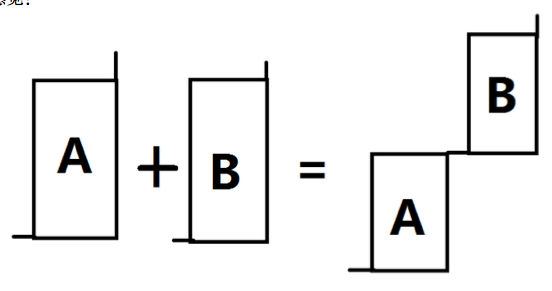
\includegraphics[width=5in]{pic/ASC43_pic1.png}

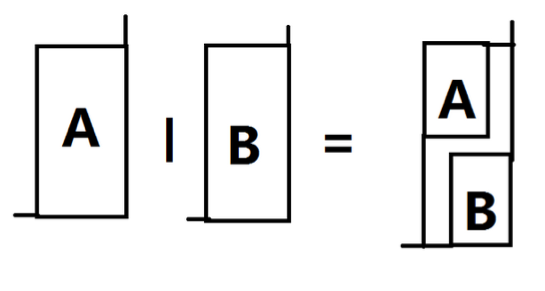
\includegraphics[width=5in]{pic/ASC43_pic2.png}

\problem{Hentium Scheduling}

\begin{description}
\item[负责] 刘炎明
\item[情况] 比赛时通过 - 103min(1Y)
\end{description}

原题,POJ3469,网络流傻逼题。考虑最小割模型,任务一排点,源到任务的边权是在处理器1上做的代价,任务到汇的边权是在处理器2上做的代价,任务之间互相连边权为通信代价的边即可,最小割即是答案,正确性显然。输出方案的话,求出从源出发的哪条边在割边集内即可。
在割边集内的条件很显然,x从源可达y从汇可达则x->y在割边集内。

\problem{IQ Test}

\begin{description}
\item[负责] 刘炎明
\item[情况] 比赛时通过 - 57min(1Y)
\end{description}

由于n只有10000,我们直接平方DP就可以了。DP时计算每个人对后面的人造成的延迟。

\problem{Jubilee Decoration}

\begin{description}
\item[负责] 邢皓明
\item[情况] 比赛时通过 - 127min(2Y)
\end{description}

$n=3$时答案为$1$,方案:全装饰成$1$即可。
$3<n \leq 6$时答案为$2$,方案:分成$\leq 3$的两条链,链上$1$和$2$各一条,中心到某一条链连$1$l的边,到另一条连$2$的边。
$n > 6$时答案为3,方案:环中心到环上点交替连1和2,环上全是3。

\problem{K. Kingdom Division 2}

\begin{description}
\item[负责] 杨越
\item[情况] 比赛时通过 - 135min(1Y)
\end{description}

由于是凸包,所以如果确定了一个点,可行的另一个点肯定是一个区间,注意到随着选定点的移动可行区间的左右端点也会单调移动,一遍扫描即可算出答案。

\problem{Least Common Ancestor}

\begin{description}
\item[负责] 邢皓明
\item[情况] 比赛时通过 - 248min(5Y)
\end{description}

先把两棵树都按照题目所说规则删到只剩根,用堆维护当前最靠右的可以直接删除的叶子对(堆中的关键字为dfs序)。然后再一个个加入,当两棵树需要加入的下一个点不同时停止,此时得到的树就是两棵树的Least Common Ancestor。

\section{总结}

本场比赛因为忽略了一道简单题(G题),而G题有20多个队伍通过,因而自废一题,最后成绩也不甚理想,但如果最后能通过F题的话还是很不错的,有点可惜。个人状态来看,我的两个队友发挥还不错,题目大多都是1Y,而我今天状态略差,没有1Y的题目,但是也算能及时查出bug。配合出现了一个失误,G题只有一个人(yy)认真读过,结果就产生了判断失误,以后要注意。

\end{document}
